\documentclass[aspectratio=169]{beamer}
%\usetheme{CambridgeUS}
%\usecolortheme{beaver}

%\usefonttheme{serif}
%\usepackage{helvet}

\usefonttheme{serif}     % Font theme: serif
%\usepackage{ccfonts}     % Font family: Concrete Math
\usepackage[T1]{fontenc} % Font encoding: T1

\setbeamersize{text margin left=42pt,text margin right=42pt} 
\setbeamertemplate{navigation symbols}{}
\setbeamertemplate{itemize items}[default]

\beamertemplatenavigationsymbolsempty

\definecolor{fore}{RGB}{51,51,51}
\definecolor{back}{RGB}{255, 254, 250}
\definecolor{title}{RGB}{ 255, 15, 0}
\definecolor{links}{RGB}{18, 168, 255}

\setbeamercolor{titlelike}{fg=title}
\setbeamercolor{normal text}{fg=fore,bg=back}
\setbeamercolor{alerted text}{fg=title}
\setbeamercolor{itemize item}{fg=title}
\setbeamercolor{enumerate item}{fg=title}
\hypersetup{colorlinks,urlcolor=links}

% for code https://kbroman.org/blog/2013/10/07/better-looking-latexbeamer-slides/
\usepackage{listings}
\definecolor{keywords}{RGB}{255,0,90}
\definecolor{comments}{RGB}{60,179,113}
\lstset{language=Python,
keywordstyle=color{keywords},
commentstyle=color{comments}emph}

% fonts
\usepackage[sc]{mathpazo}


% title info
\title{\textbf{Cars, Roads, \& Highways}}
\subtitle{\textbf{GGR424 - Transportation Geography \& Planning}}
\author{Jeff Allen}
\institute{University of Toronto}
\date{January 17, 2022}


\begin{document}
	
\begin{frame}
	\titlepage	
\end{frame}



\begin{frame}
\textbf{Today:}
\begin{itemize}
	\item Cars \& Highways - A Brief History
	\item Road Networks \& Hierarchy
	\item Accessibility \& Mobility
	\item Induced Demand, Highway Expansion
	\item Activity - Debate?
\end{itemize}
\end{frame}



\begin{frame}
	
	Mode Share for all trips in the GTHA (Greater Toronto \& Hamilton Area)
	
	\vspace{4mm}
	
	\begin{figure}
		\centering
		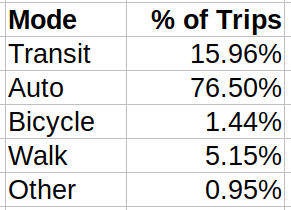
\includegraphics[width=0.3\linewidth]{images/mode_share_gtha_2016.png}
		\tiny{Source: 2016 Transportation Tomorrow Survey}
	\end{figure}
	
\end{frame}




\begin{frame}
	
	\begin{figure}
		\centering
		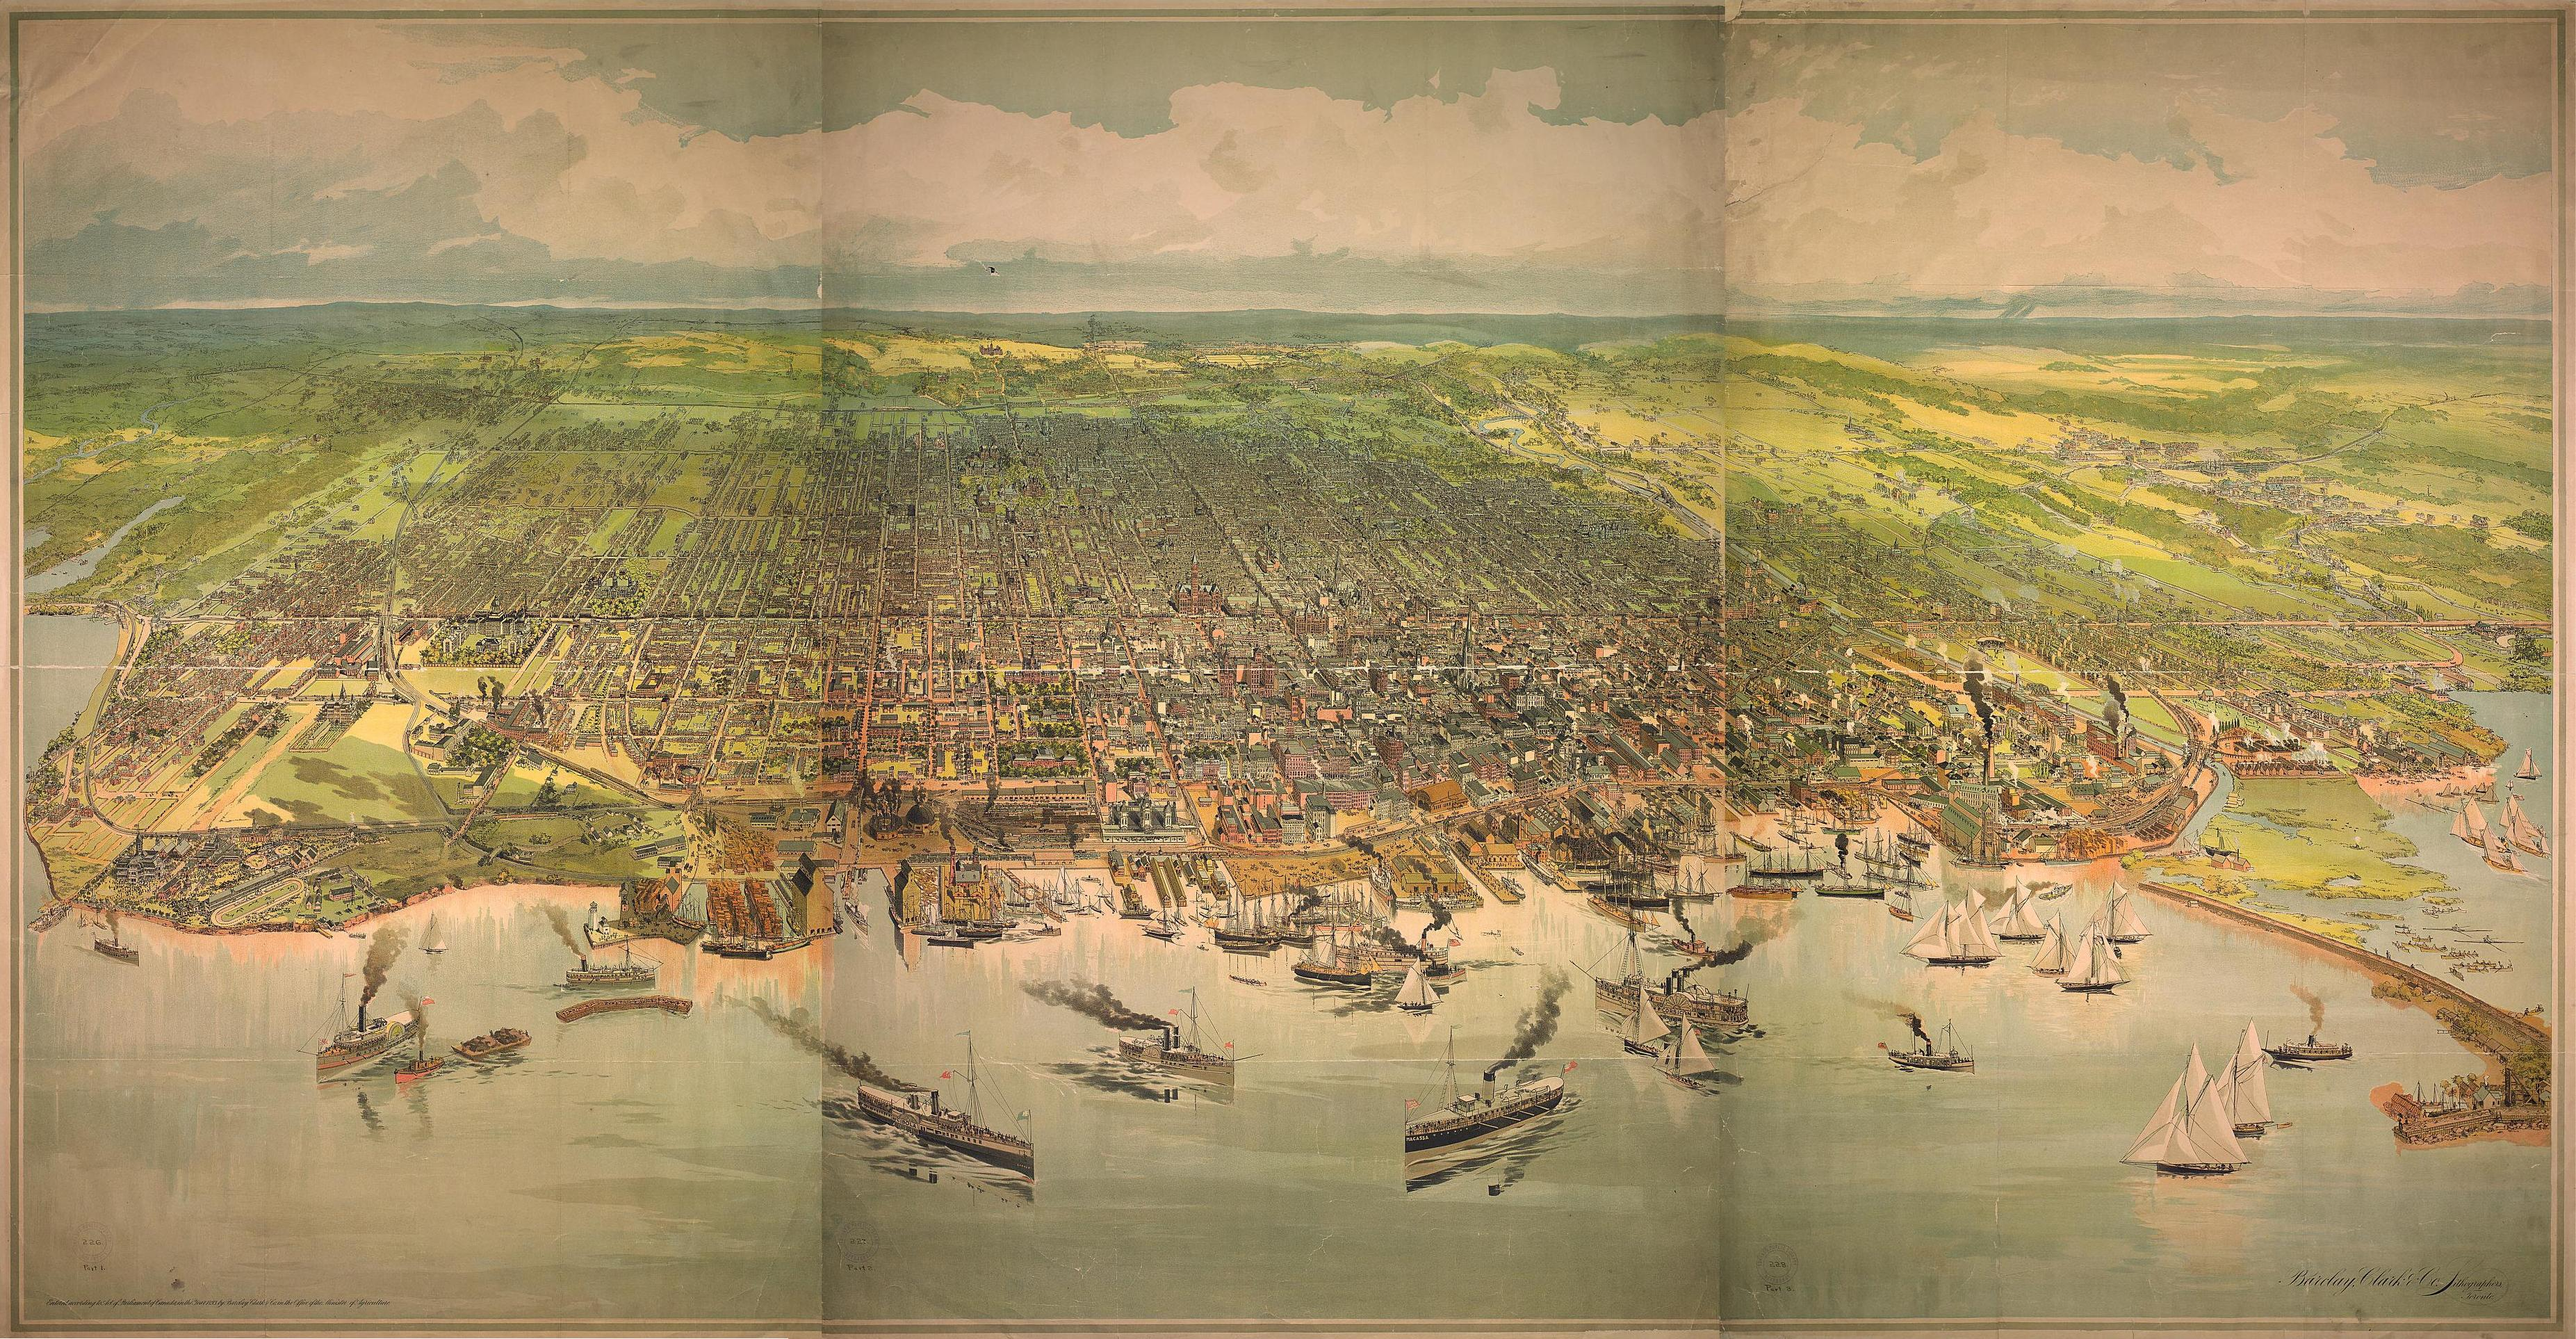
\includegraphics[width=1.1\linewidth]{images/toronto_1893.jpg}
		
	\end{figure}
	\tiny{Via UofT Map \& Data Library \url{https://maps.library.utoronto.ca/datapub/digital/NG/historicTOmaps/1893BarclayClark.Chromolithograph_of_City_of_Toronto.JPG}}
	
\end{frame}










\begin{frame}
	
	\begin{figure}
		\centering
		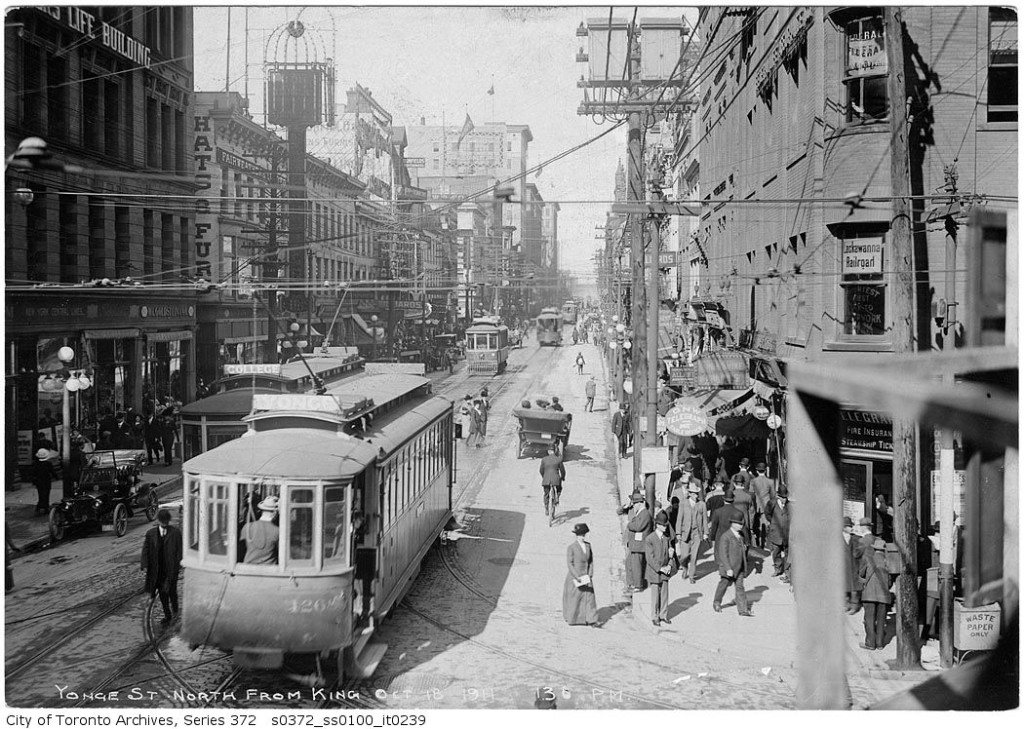
\includegraphics[width=0.8\linewidth]{images/yonge-north-from-king-1911.jpg}
		
	\end{figure}

	% what see?
	
\end{frame}



\begin{frame}
	
	\begin{figure}
		\centering
		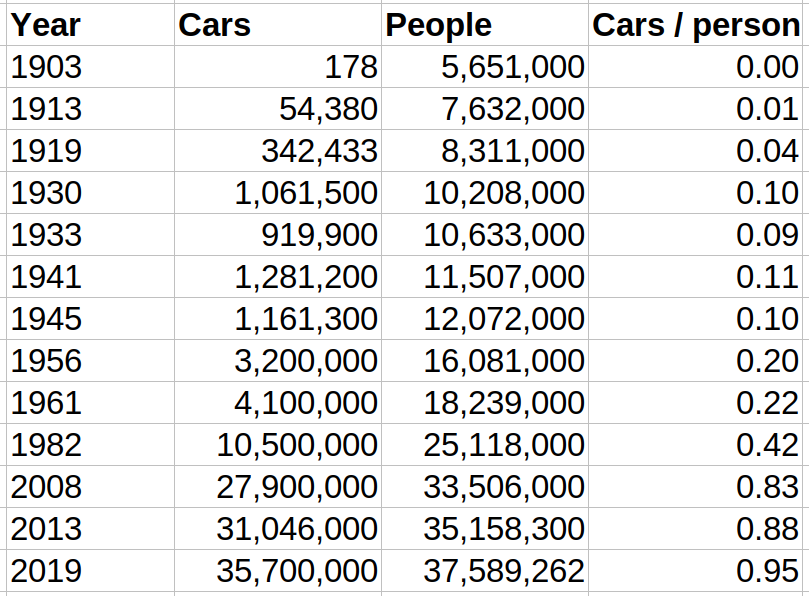
\includegraphics[width=0.6\linewidth]{images/cars_ppl_canada.png}
		
	\end{figure}
	
	\tiny{
		Sources:
		
		- McNally, Larry. “Roads, Streets, and Highways,” in Building Canada: a history of public	works
		
		- \url{https://www.statcan.gc.ca/en/topics-start/automotive}	
}
	
\end{frame}




\begin{frame}
	
	\begin{figure}
		\centering
		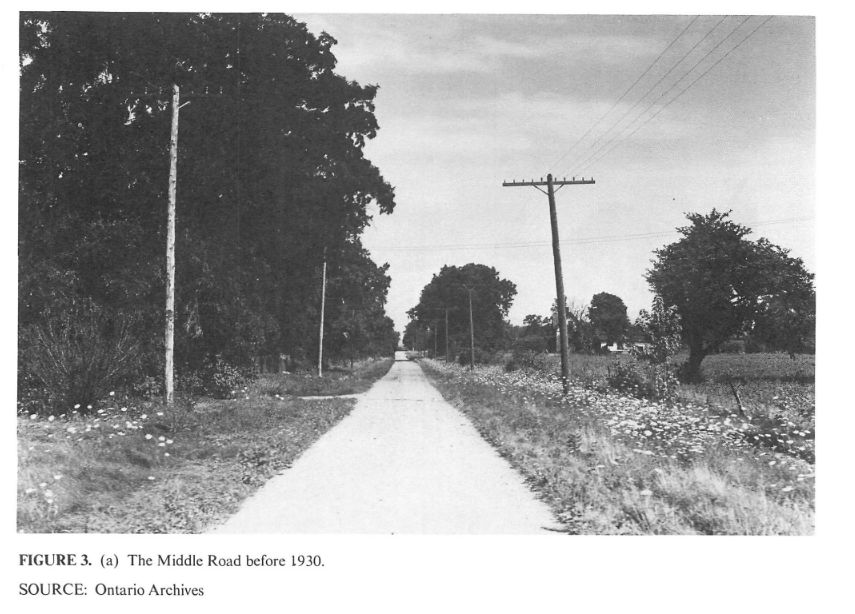
\includegraphics[width=0.8\linewidth]{images/qew_1930.png}
		
	\end{figure}
	\tiny{The Queen Elizabeth Way: Public Utility Versus Public Space = \url{https://www.erudit.org/en/journals/uhr/1900-v1-n1-uhr0860/1018953ar.pdf}}
	
\end{frame}





\begin{frame}
	
	\begin{figure}
		\centering
		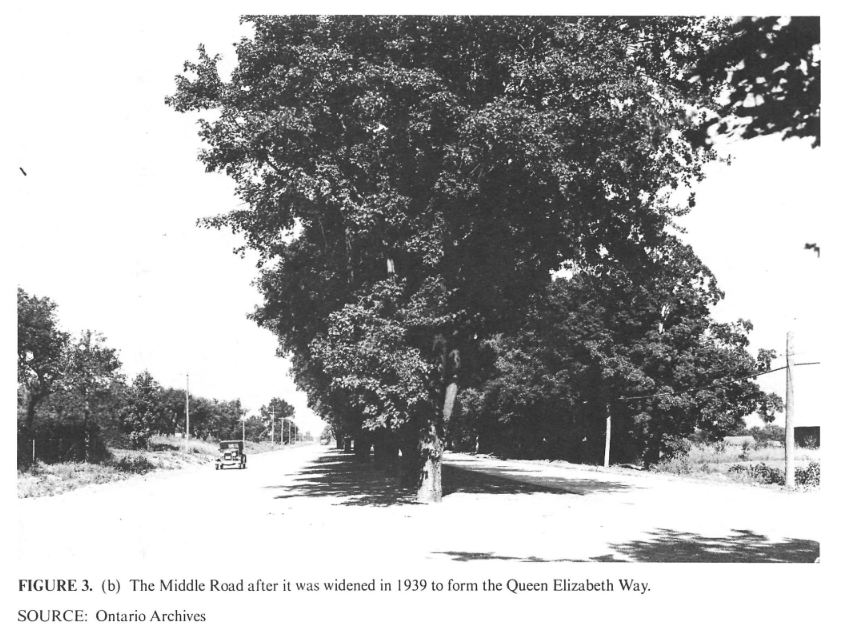
\includegraphics[width=0.8\linewidth]{images/qew_1939.png}
		
	\end{figure}
	\tiny{The Queen Elizabeth Way: Public Utility Versus Public Space = \url{https://www.erudit.org/en/journals/uhr/1900-v1-n1-uhr0860/1018953ar.pdf}}
	
\end{frame}


\begin{frame}
	
	\begin{figure}
		\centering
		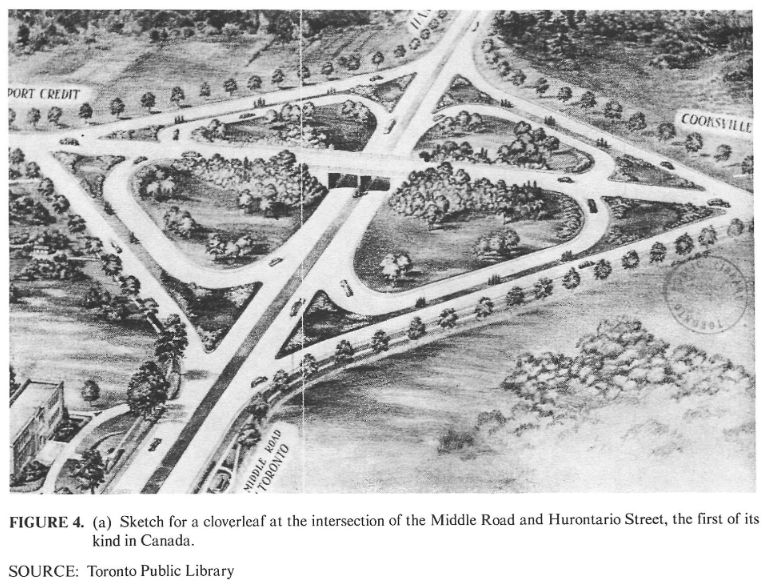
\includegraphics[width=0.8\linewidth]{images/qew_highway10.png}
		
	\end{figure}
	\tiny{The Queen Elizabeth Way: Public Utility Versus Public Space = \url{https://www.erudit.org/en/journals/uhr/1900-v1-n1-uhr0860/1018953ar.pdf}}
	
\end{frame}





\begin{frame}
	
	\begin{figure}
		\centering
		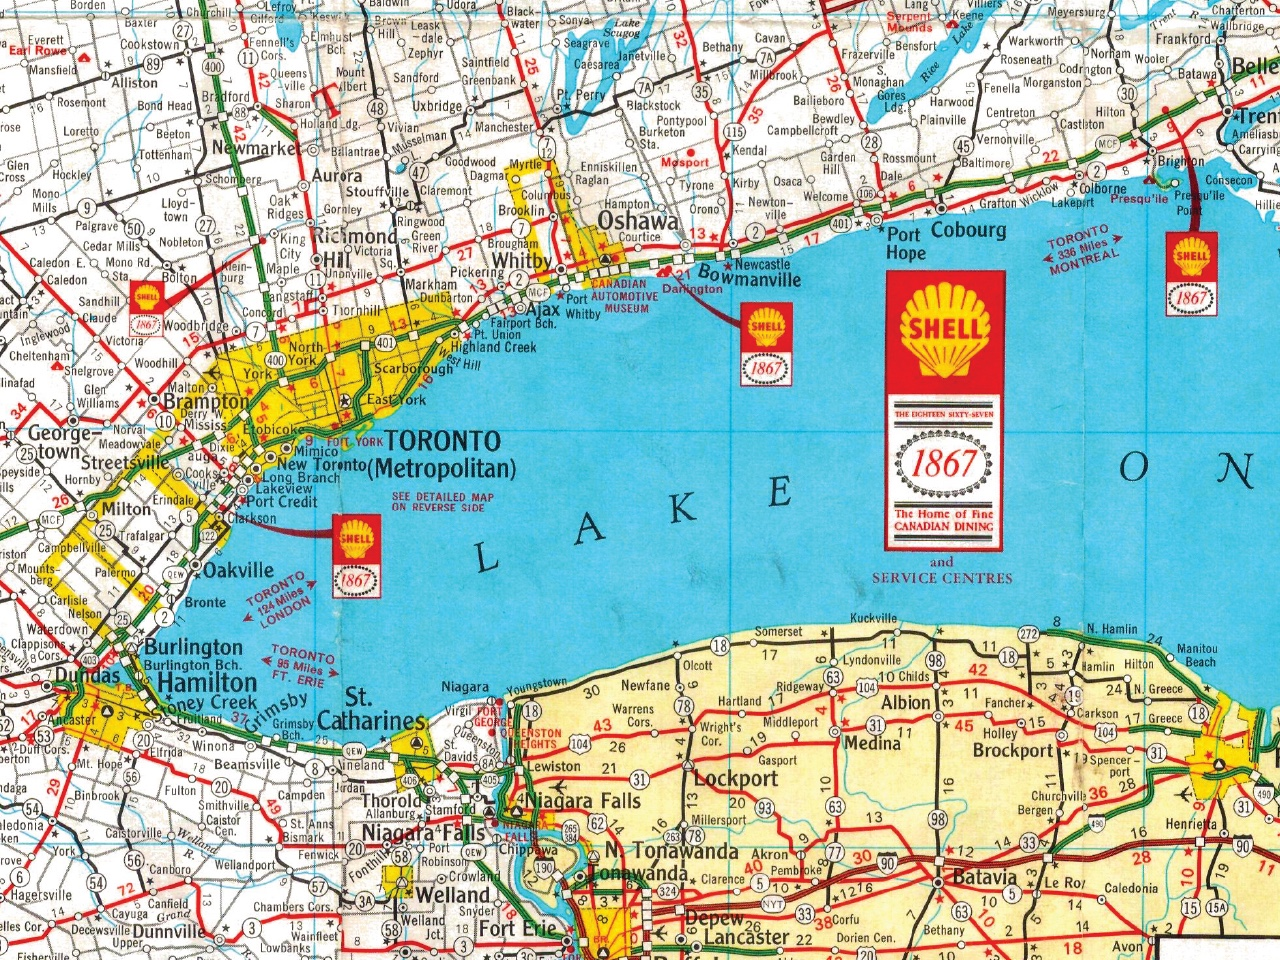
\includegraphics[width=0.85\linewidth]{images/shell_map_ontario_1968.jpg}
		
	\end{figure}
	\tiny{\url{https://www.vice.com/en/article/4xay73/the-little-known-capitalist-history-of-the-highway-map}}
	
\end{frame}


\begin{frame}
	
	 \textbf{Road Hierarchy} \\
	 
	 \begin{itemize}
	 	\item Ranking of roads based on their functions and characteristics
	 	\item Historically (and still usually) based on vehicle speeds and throughput
	 	\item  e.g. common hierarchy
	 	\begin{enumerate}
	 		\item Highway / Motorway
	 		\item Major Arterial
	 		\item Minor Arterial
	 		\item Collector
	 		\item Local
	 	\end{enumerate}
 		\item Used for design and maintenance of road networks
	 \end{itemize}
	 

	
\end{frame}




\begin{frame}
	
	Current Road Hierarchy in Toronto:
	
	\begin{figure}
		\centering
		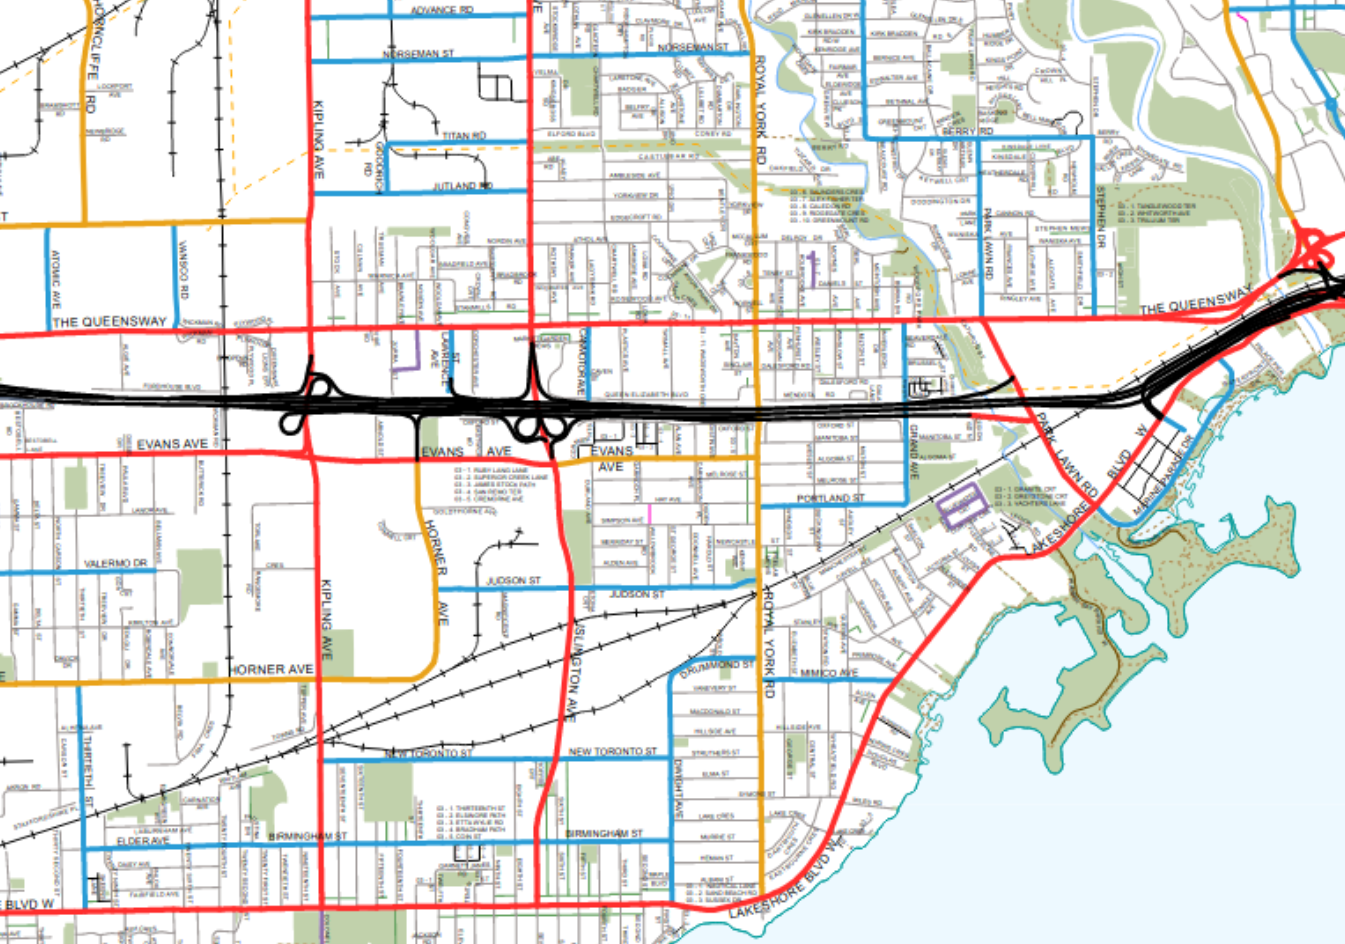
\includegraphics[width=0.85\linewidth]{images/tor_road_heir.png}
		
	\end{figure}
	\tiny{\url{https://www.toronto.ca/services-payments/streets-parking-transportation/traffic-management/road-classification-system/about-the-road-classification-system/}}
	
\end{frame}





\begin{frame}
	\textbf{Key Concepts in Urban Transportation}
	\normalsize
	\vspace{4mm}
	\begin{itemize}
		\item Travel Demand
		\item Activity Participation
		\item Utility
		\item Travel Behaviour
		\item \textbf{\underline{Mobility}}
		\item \textbf{\underline{Accessibility}}
		% \item Transport \& Land Use
		% \item Mobility VS Accessibility
	\end{itemize}
\end{frame}



\begin{frame}
	
	\textbf{Mobility}
	\begin{itemize}
		\item The ease of travelling
	\end{itemize}

	\textbf{Accessibility}
	\begin{itemize}
		\item The ease of reaching destinations
		\item Depends on mobility, but also land-use (i.e. the proximity of destinations)
	\end{itemize}
	
\end{frame}




% mobility accessibility


% Toronto highway expansion mid 20th

% stopped, partly

% Spadina subway



\begin{frame}
	\textbf{Next Week} 
	
	\vspace{4mm}
	
	Cycling \& Walking:
	
	\begin{itemize}
		
		
		
		\item Walking and cycling in the city
		
		\item Health benefits of active travel
		
		\item Safety issues
		
		\item Streets as public space
		
		\item Designing complete streets
		
		
		
	\end{itemize}

\end{frame}




\end{document}